
\section{Introduction}
% Based on this Google Doc: 
% https://docs.google.com/document/d/1e4_mH7MMYO3bad9BoknrRlWR4jOcKNOFV8UyYLU5kPA/edit

% Apple and Google recently joined forces to develop a new privacy-preserving mobile contact tracing protocol that leverages the hardware in all modern phones to automate contact tracing without revealing information about their users.  
% Despite its potential, this new protocol and how it is being deployed has created tension with governments around the world who are legitimately concerned that it will hinder manual contact tracing and undermine their ability to manage the spread of the virus. 

% Apple and Google have adopted a decentralized approach arising out of academic research that seeks to preserve privacy.   
% All contact identification and risk analysis is done locally on individuals phones without revealing where the contact event took place or the identity of the infected individual.   
% The protocol does not use location information and instead relies on the low-power Bluetooth hardware present on all modern phones.  
% The protocol is entirely opt-in and the only information that is ever shared with public authorities are non-identifying cryptographic keys provided by the COVID-positive individuals.

% However, many governments and public health authorities are advocating for a centralized approach where they maintain a record of the locations and interactions between individuals and can compute potential exposures from confirmed individuals and notify people directly.  Furthermore, location information allows them to better understand where and how the disease is spreading, so they can take preventative measures. While the utility of centralized and attributable contact tracing is critical to re-opening the world’s economy, it also raises profound concerns for civil liberties and personal privacy.

% The tech giants have taken an unprecedented position -- essentially dictating public policy by prohibiting contact tracing apps that rely on the new protocols from collecting location information.  Further, they are restricting access to the new contact tracing APIs to national governments and permitting only one app per country or region.  This decision circumvents the local governments, tribal organizations, and community health services that are often most aware of the needs of their communities and the nexus of existing manual contact tracing efforts.  Meanwhile, governments who have attempted to launch their own contact tracing apps have failed due to restrictions imposed by the Apple and Google operating systems.

% Path Forward: Both of these positions have rational basis, significant merits, and faults.  Generally, all would agree that we want to both preserve civil liberties and improve the efficacy of public health processes for detecting, containing, and mitigating the spread of the virus.  Our phones and our cooperation can be an essential part of the solution. It is well established that the Apple and Google approach is only effective if a large fraction of the population participates, but without very clear protection of personal privacy, the needed level of participation will not occur in a free society.  

% Surprisingly, with two simple measures, we can return authority to local communities without fragmenting contact tracing efforts, support manual contact tracing efforts, and provide visibility into the spread of disease all within the proposed privacy-preserving decentralized approach outlined by Apple and Google. In the rest of this article, we outline these two simple measures and how they both improve contact tracing while also preserving individual privacy.



%%%%%%%%%%%%%%%%%%%%
% START LIGHTHOUSE %
%%%%%%%%%%%%%%%%%%%%

% Governments around the world have become increasingly frustrated with tech giants dictating public health policy. The software created by Apple and Google enables individuals to track their own potential exposure through collated exposure notifications. However, the same software prohibits location tracking, denying key information needed by public health officials for robust contract tracing. This information is needed to treat and isolate COVID-19 positive people, identify transmission hotspots, and protect against continued spread of infection.


Apple and Google have adopted a decentralized approach to mobile contact tracing that prioritizes individual privacy~\cite{agen}. Under the Apple-Google Exposure Notification (AGEN) protocol (see Fig.~\ref{fig:contact_tracing}), individual phones determine if the user has been exposed, without revealing \emph{the identity of the infected individual} and \emph{where the contact event took place}
The AGEN protocol is related to contemporaneously proposed protocols including PACT and DP-3T~\cite{pact,dp3t}.
Like these other protocols, the AGEN protocol does not use location information. 
Instead, it relies on the Bluetooth radios present on all modern phones to detect proximity with others. 
Beyond not collecting Protected Health Information (PHI), the decentralized approach retains the non-PHI on the phone, allowing individuals to determine risk locally on their device.

\begin{figure}[t]
    \centering
    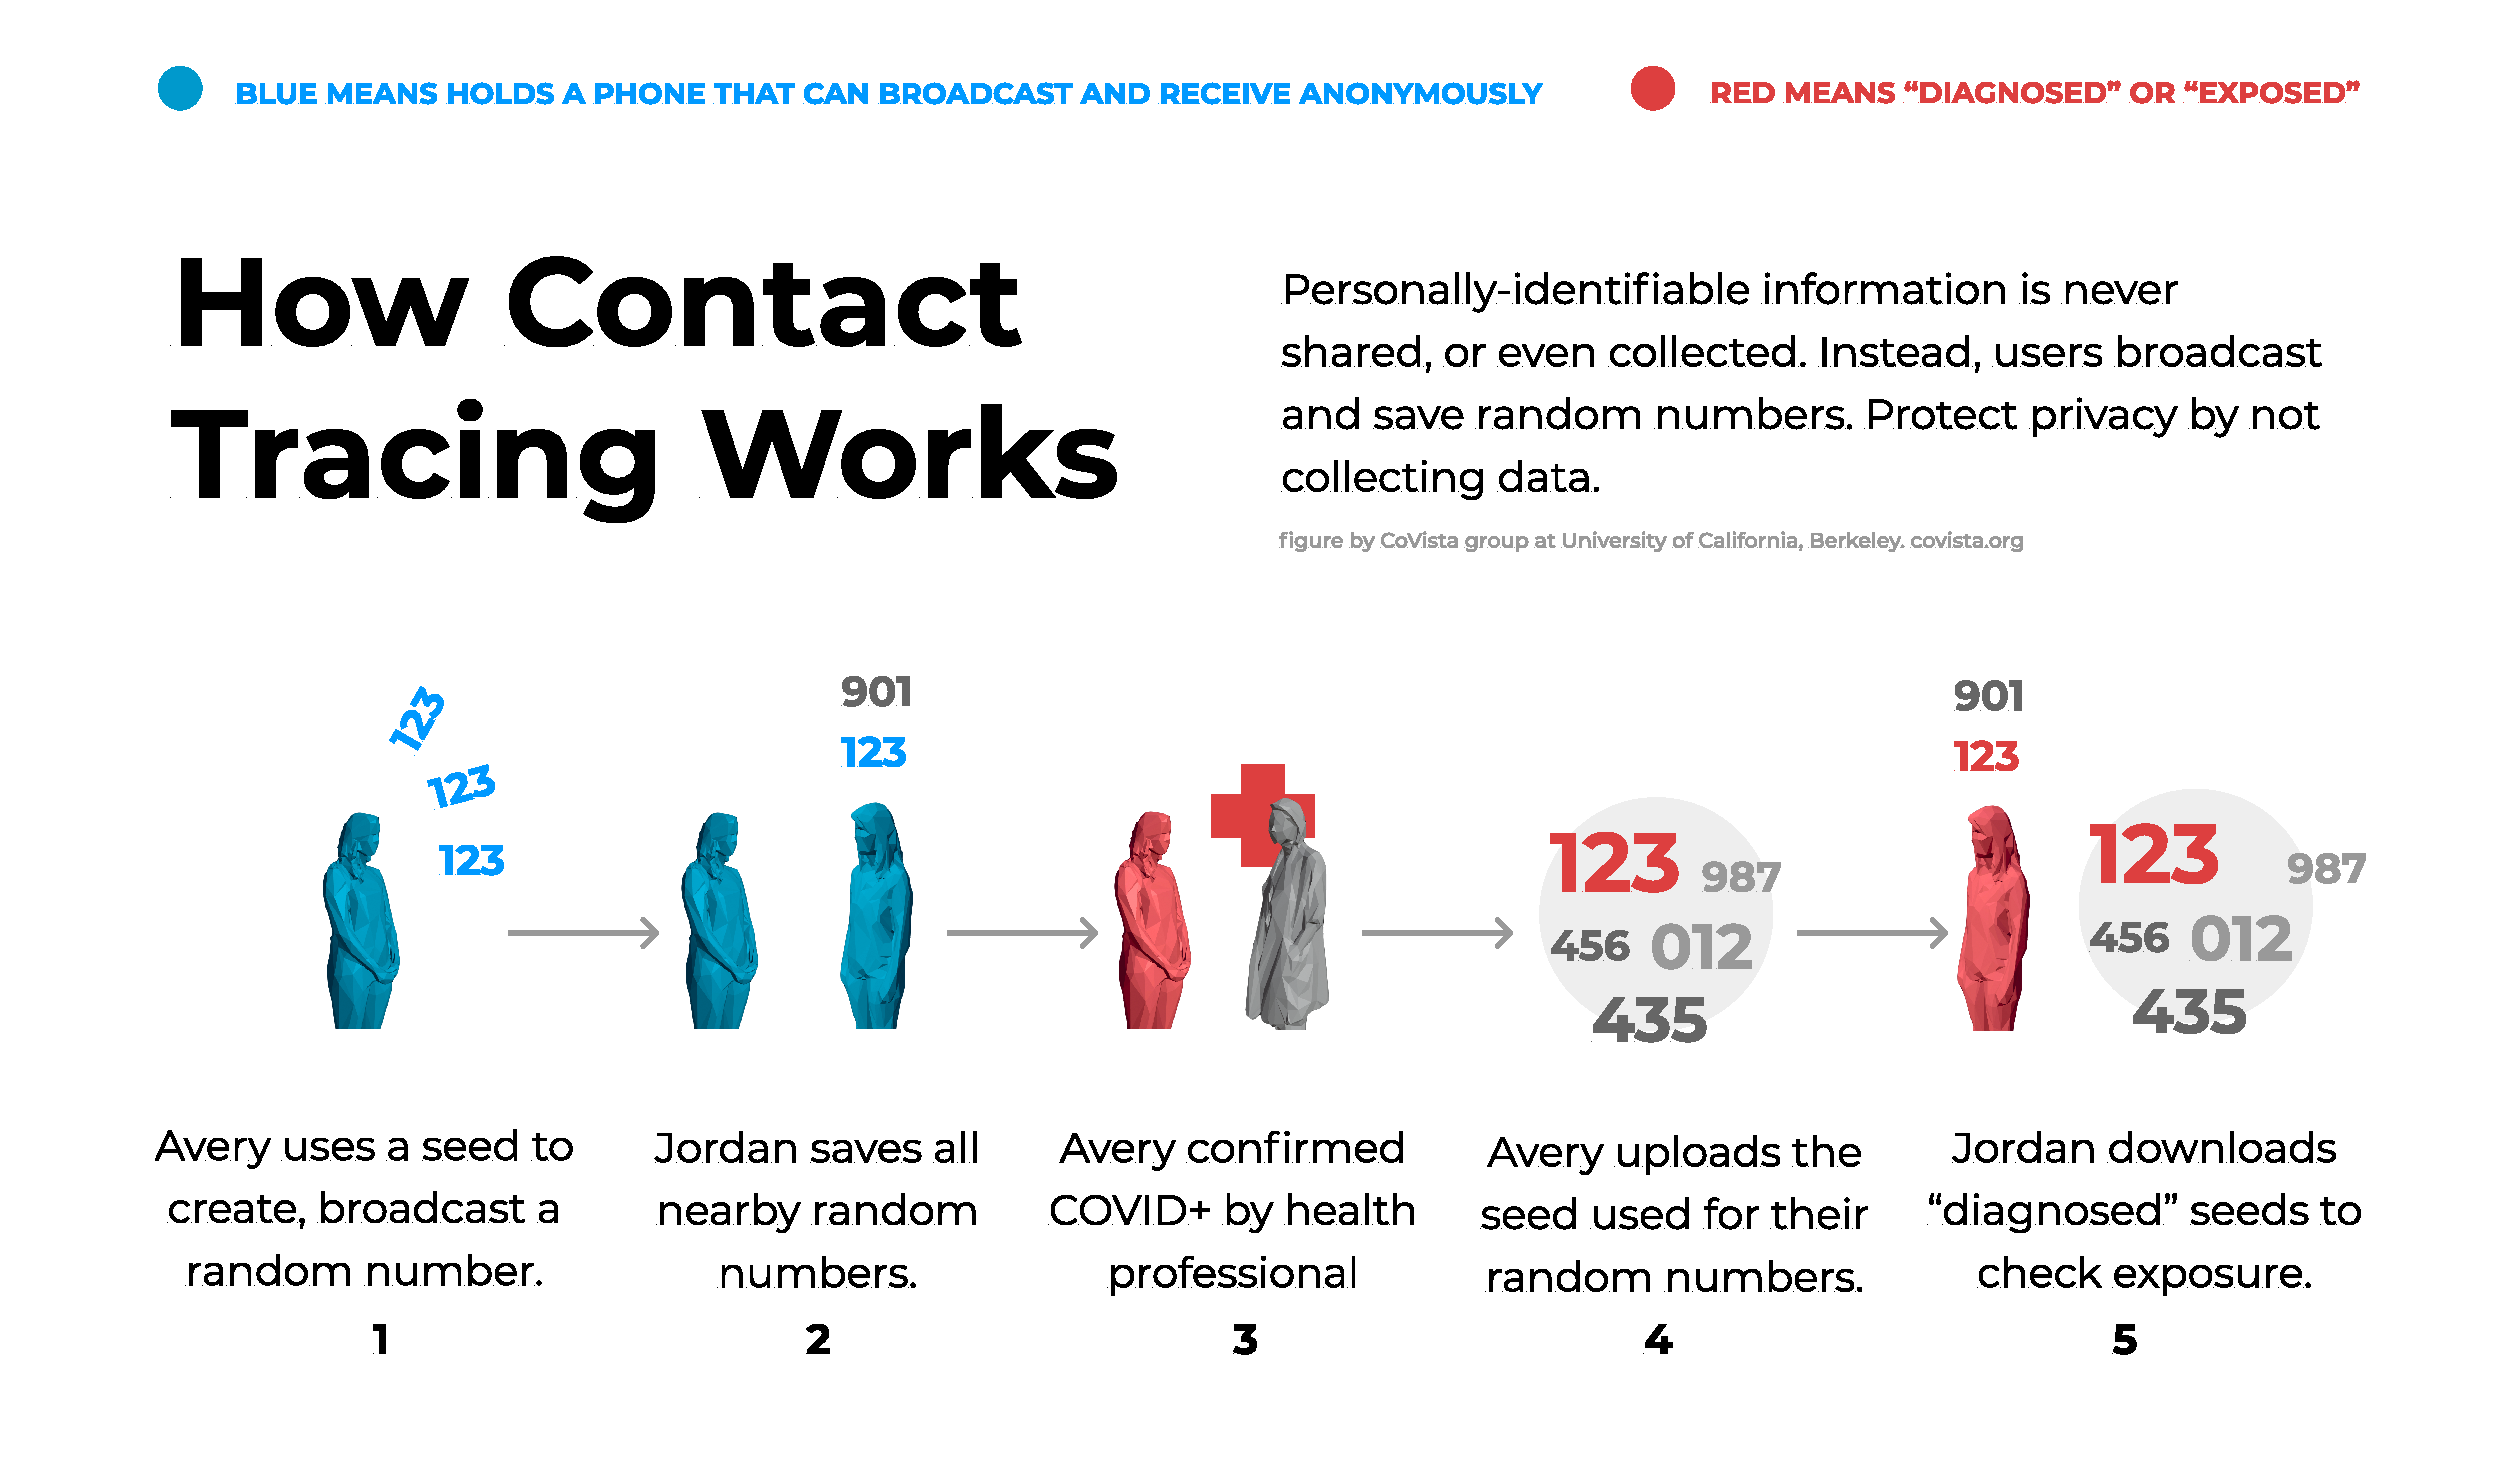
\includegraphics[width=0.8\textwidth]{figs/how_contact_tracing_works.pdf}
    \caption{Apple-Google Exposure Notification (AGEN) Protocol Overview.}
    \label{fig:contact_tracing}
\end{figure}

Governments and public health authorities want to understand where and how the disease is spreading, so they can take preventative measures.  
They also want to be able to use mobile contact tracing to augment existing manual contact tracing efforts.
With these goals in mind, governments advocate for a centralized approach, whether national or regional, where they maintain records of each person’s locations and interactions. 
This allows governments to determine exposures and notify people directly, as timeliness reduces spread. 
While centralized contact tracing may offer utility critical to re-opening the world’s economy, it raises profound concerns for civil liberties and personal privacy.
Government efforts that avoid reliance on the industrial Exposure Notification offerings have run into a host of failings, including reliability, power drain, interoperability, and participation.

Apple and Google have taken an unprecedented position -- essentially dictating public policy, not just by requiring the decentralized approach, but also by prohibiting contact tracing apps from collecting location information.
Further, they are restricting access to the new contact tracing APIs to national governments and permitting only one app per country or region. 
This decision circumvents the local governments, tribal organizations, and community health services that are often most aware of existing manual contact tracing efforts and the needs of their communities.  
Meanwhile, government contact tracing apps have failed due to restrictions imposed by AGEN.

In this article, we present two simple measures that enable the AGEN protocol to support manual contact tracing efforts, provide visibility into the spread of disease, and return authority to local communities all while preserving privacy within the Apple and Google framework. 
\begin{enumerate}
\item \textbf{Treat places as people.} Endow public places with the same privacy-preserving technology used to monitor exposure for individuals.
\item  \textbf{Nation-scale data, not apps and processes.} Build a common backend for the AGEN protocol that spans apps and governmental boundaries.
\end{enumerate}

In the rest of this article, we describe these two simple measures and how they both improve contact tracing while also preserving individual privacy.

\subsection*{Lighthouse: Treat Places as People}
\begin{figure}[h]
    \centering
    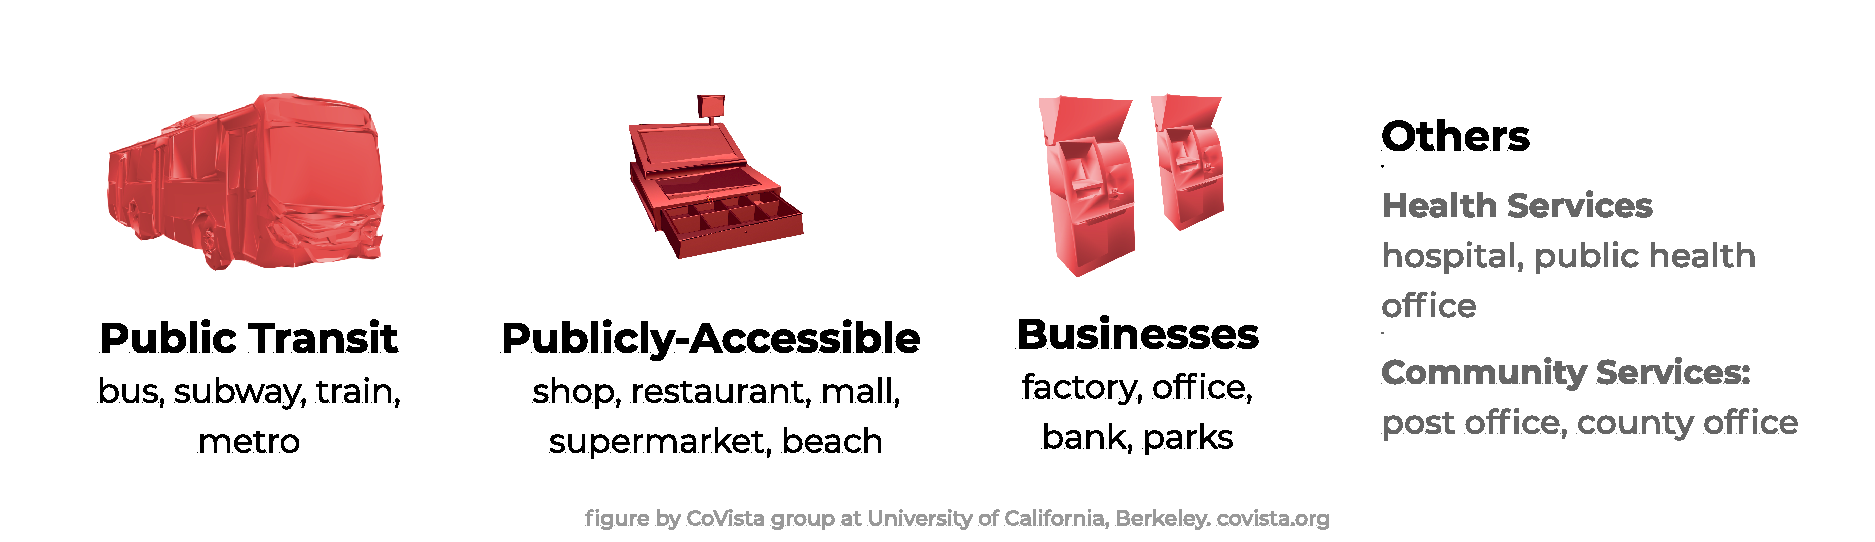
\includegraphics[width=\textwidth]{figs/places.pdf}
    \caption{Lighthouses can extend the AGEN protocol to physical places}
    \label{fig:placesExamples}
\end{figure}

If we treat public places as people, we can use the AGEN protocol to (a) understand COVID-19 exposures across space, (b) integrate with manual contact tracing, and (c) do so with the same privacy-sensitive protocol. To treat places as people in AGEN, simply attach mobile phones or specialized low-cost beacons to publicly accessible places (e.g., county services, stores, buses).  
Like a lighthouse, these devices help communicate risk associated with places.  
Well-positioned, they can offer robust proximity detection, can detect their exposure, and can convey aspects the risk that represents.

By choosing to share their locally computed exposure risk with public health authorities through the AGEN protocol, owners of publicly-accessible places can aid in mitigating virus spread. 
Alternatively, if a place is identified through traditional, manual contact tracing, the place can still anonymously participate in the AGEN protocol, notifying others without revealing where they were exposed. 
Treating places as people empowers stewards of public spaces to collaborate with public health authorities to help mitigate the spread of disease without jeopardizing the privacy of patrons or the reputation of the public spaces.
This procedure can facilitate detection of exposure from a non-participating individual while improving anonymity over manual contact tracing methods.  Going even further, such places could provide other means of beaconing that do not involve smartphones, such as QR code displays, codes on receipts and so on.

\subsection*{COVID Commons: A Nation-scale Data Backend}

Rather than “one app per nation,” a better solution would be to provide a common privacy-preserving data exchange across apps and administrative boundaries — a Commons.  This would allow societal structures and innovation, rather than corporate policy, to determine how the app ecosystem should evolve.  It is very likely that participation will be greatest if the apps are available through local organizations (e.g., tribal organization, university campus) that individuals trust.   A common privacy-preserving data exchange is already compatible with the AGEN protocol.

\begin{figure}[h]
    \centering
    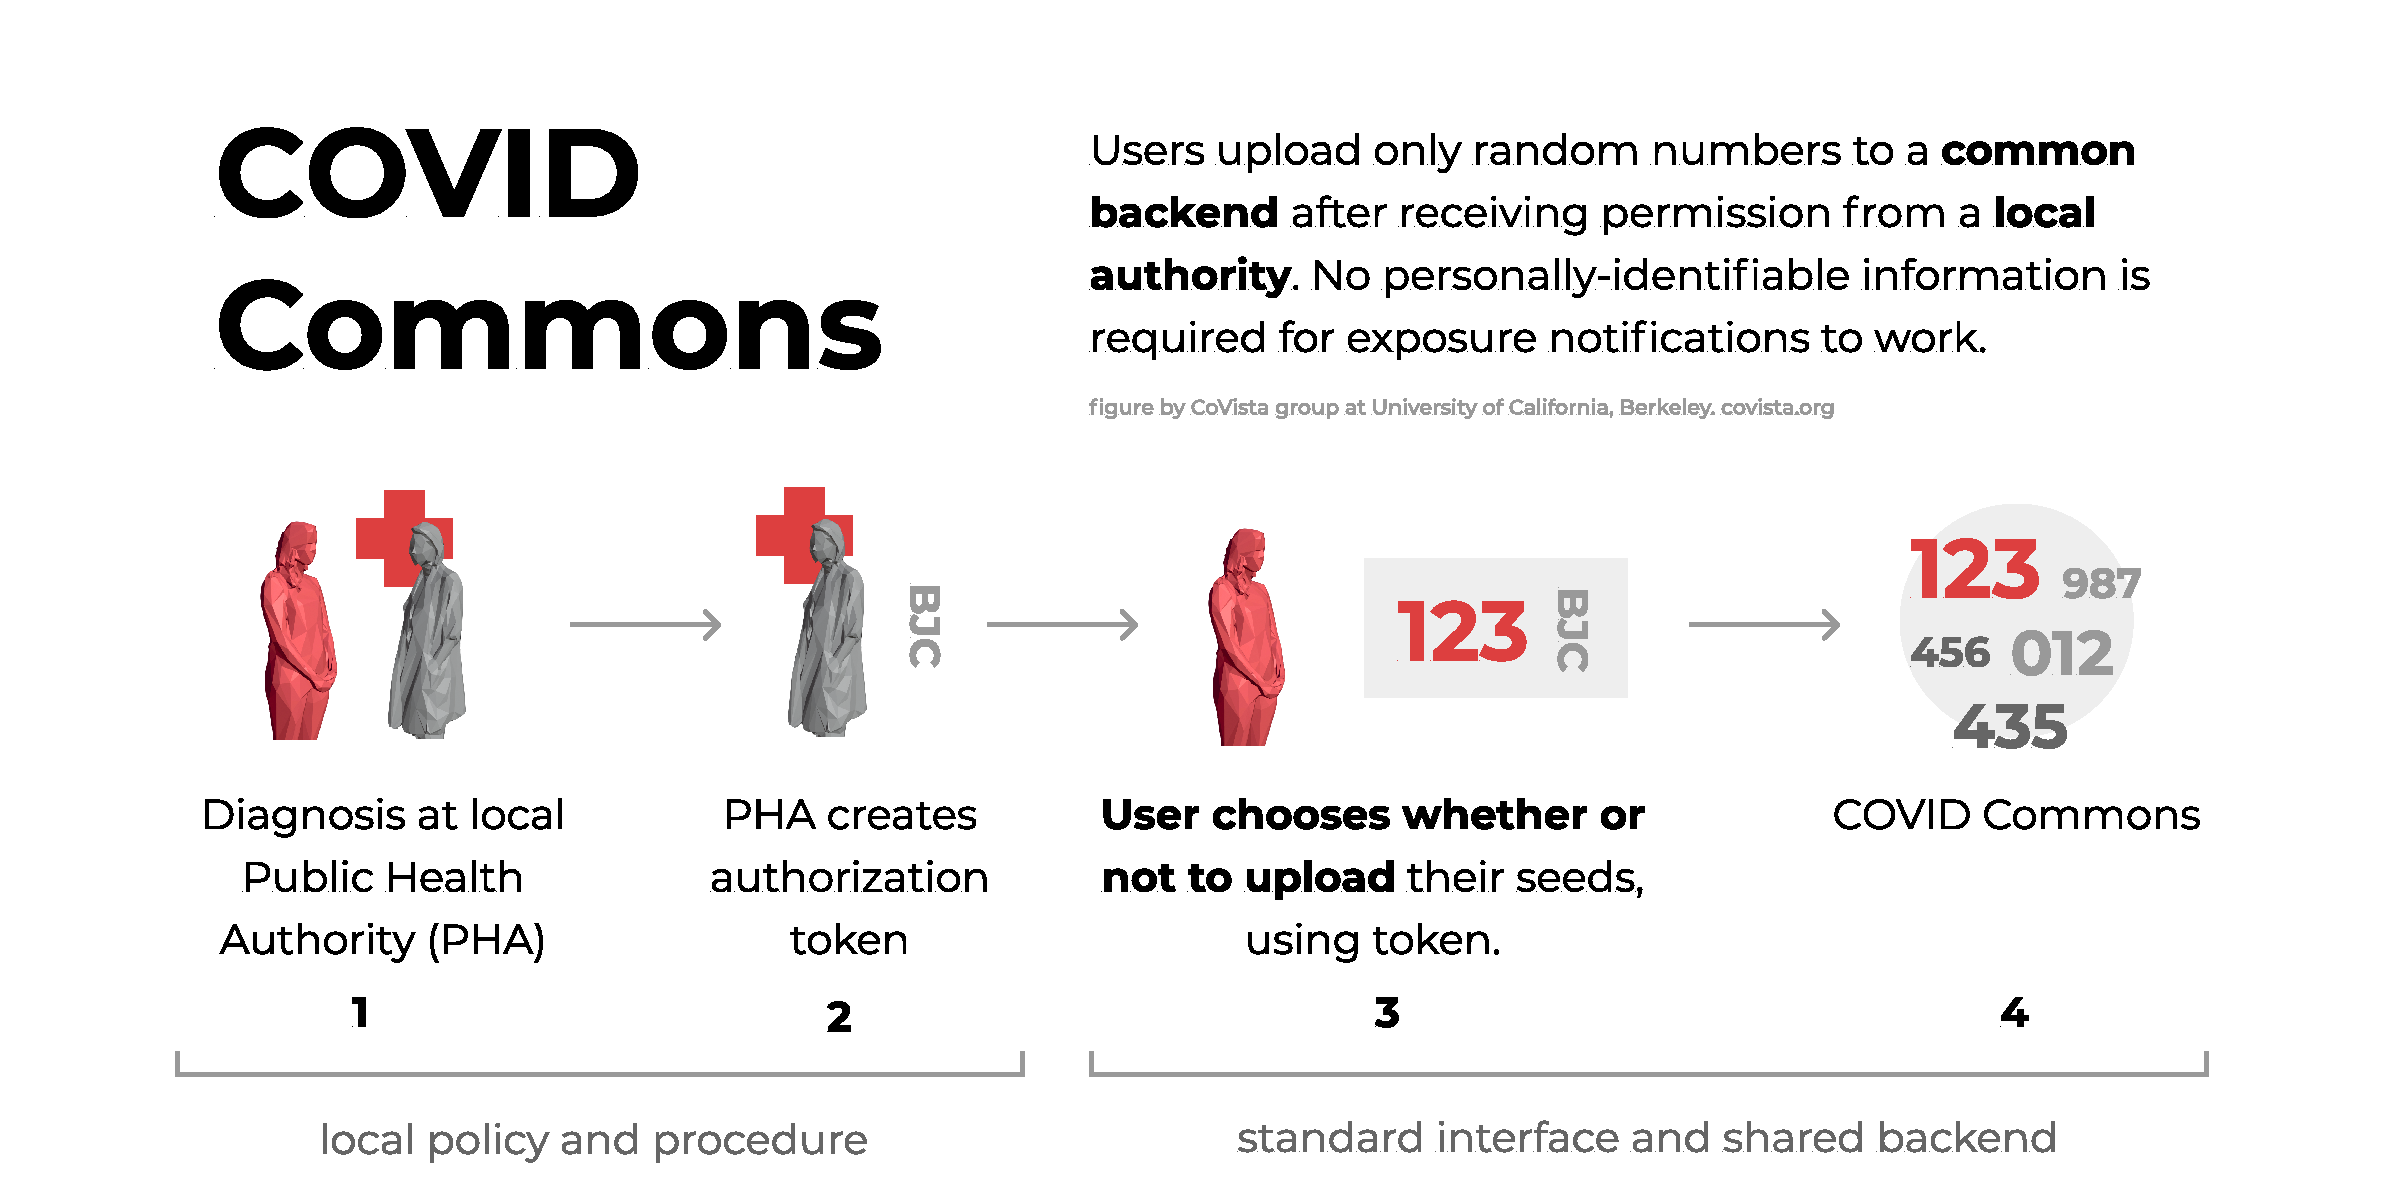
\includegraphics[width=\textwidth]{figs/covid_commons.pdf}
    \caption{Covid Commons exposure notification process.}
    \label{fig:commoms}
\end{figure}

When an individual tests positive and they engage in a conventional contact tracing interview with a public health professional. The professional obtains an authorization so the individual, on an opt-in basis, can share their anonymous exposure information.  Public health professionals serve to protect the integrity of the information in the Commons without exposing any patient data or medical data. \shankari{individual obtains authorization from professional. "an authorization"? is something like "token" missing?}

Their actions are quite similar to publishing counts of cases, statistics and demographic information, as is done today.  The Commons might be hosted by governmental or NGO structures, based on national or regional policy.  A diverse and innovative app ecosystem can grow to meet the needs of individuals and agencies.

In the remainder of this article we describe both these technical solutions in greater detail.  
We have organized each section to be relatively self-contained.
